\noindent
In this Section the user interface design, already presented in  \textit{Section 3.1.1 User Interfaces} of \textit{Requirements and Analysis Specification Document} with several mockups, is explained in more detail. A special attention is focused on the interaction between the user and the system, and on how the mockups are correlated to each other.
\bigbreak
\noindent
\begin{enumerate}
\item[•]{\Large Data4Help}
\bigbreak
\noindent
Third parties can interact with Data4Help system through a website from which they can make the several kind of requests.
\begin{figure}[H]
        \centering
          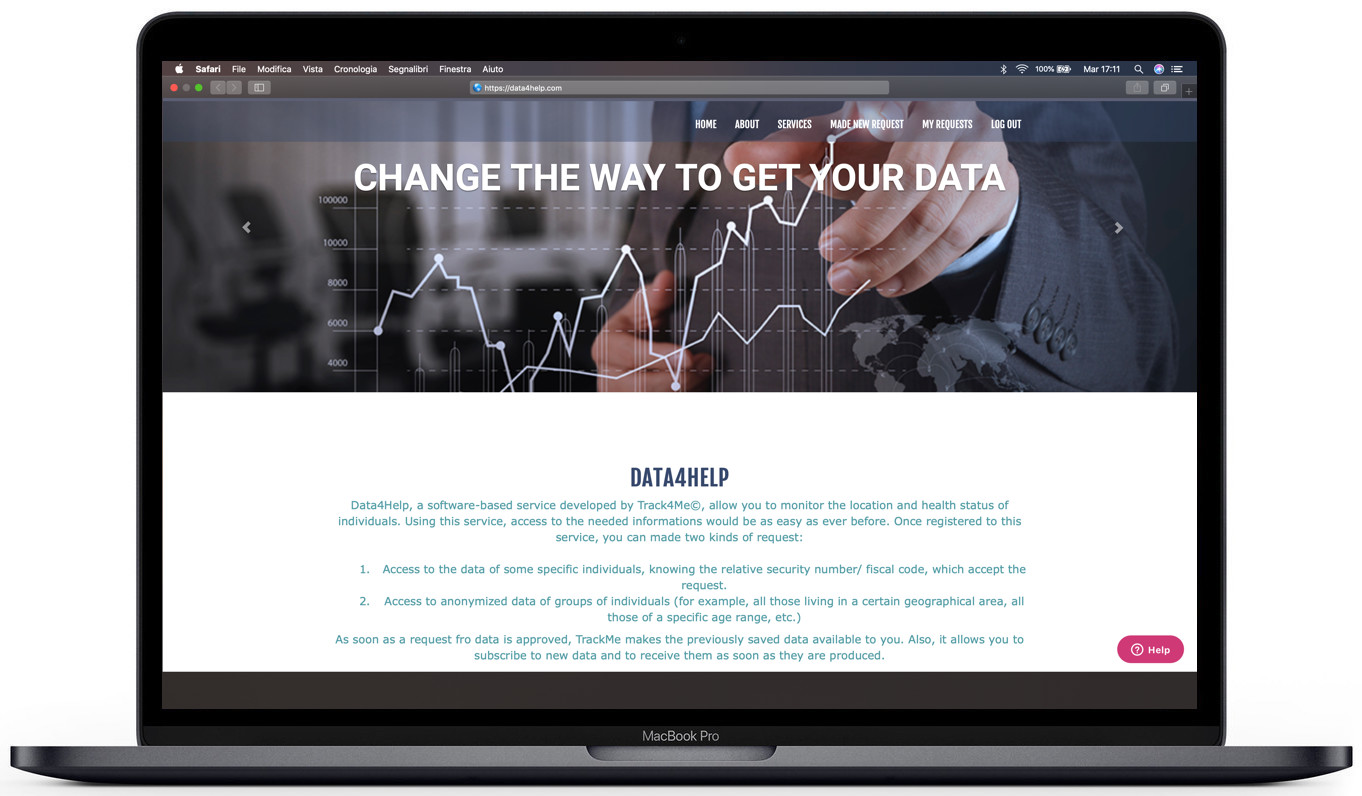
\includegraphics[scale = 0.33]{Images/Mockups/Homepage.jpg}
          	\caption{Data4Help's Homepage Mockup}
\end{figure}
This is the homepage of Data4Help's website, reachable from the user's browser by the link \texttt{www.data4help.com}. In the homepage it is possible to read a brief overview of the service offered by Track4Me. Several actions are possible from here clicking on the different buttons present in the header {\textcolor{Blue}{\textbf{HOME}}}, {\textcolor{Blue}{\textbf{ABOUT}}}, {\textcolor{Blue}{\textbf{SERVICES}}}, {\textcolor{Blue}{\textbf{MAKE NEW REQUEST}}} and, since the user is already logged into the system, also the options {\textcolor{Blue}{\textbf{MY REQUESTS}}} and {\textcolor{Blue}{\textbf{LOG OUT}}} are available. Besides the options that can be selected in the header, scrolling down the page it is possible to select a button to directly make a monitoring request. 
\bigbreak
\noindent
Clicking on {\textcolor{Blue}{\textbf{MY REQUESTS}}} a list of all the historical requests will appear, both the approved and the denied ones and also the requests waiting for the approval. For the approved ones it is also possible to see the relative answers containing all the request information.
\clearpage

\begin{figure}[H]
        \centering
          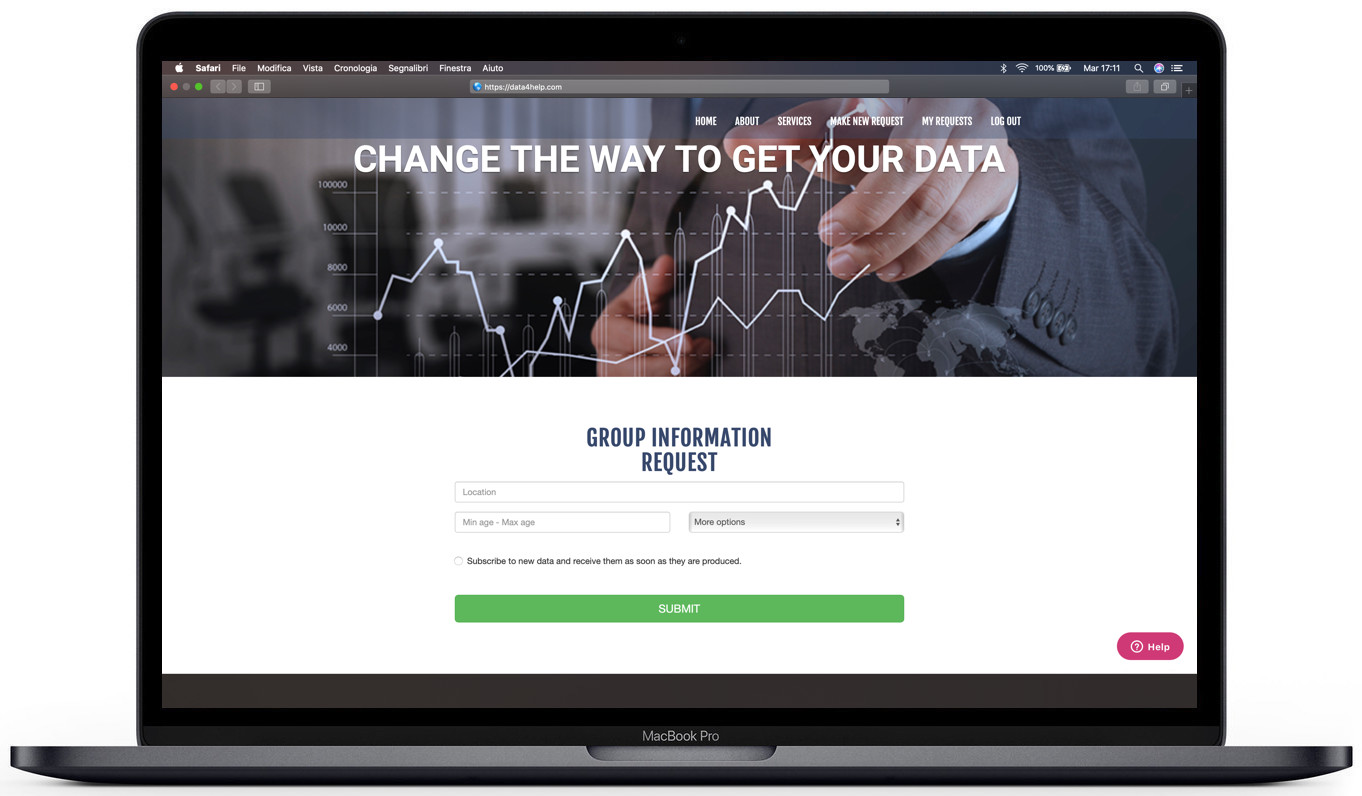
\includegraphics[scale = 0.33]{Images/Mockups/IndividualRequest.jpg}
          	\caption{Individual Request Form Mockup}
\end{figure}
Clicking on {\textcolor{Blue}{\textbf{MAKE NEW REQUEST}}}, the website loads another page where the third party is asked to select an option between {\textcolor{Blue}{\textbf{INDIVIDUAL MONITORING REQUEST}}} and {\textcolor{Blue}{\textbf{GROUP MONITORING REQUEST}}}. Clicking on the first option the system loads a new page containing the form to make an individual monitoring request. Once filled the security number's field it is possible to submit the request pressing the {\textcolor{Blue}{\textbf{SUBMIT}}} button.
\clearpage

\begin{figure}[H]
        \centering
          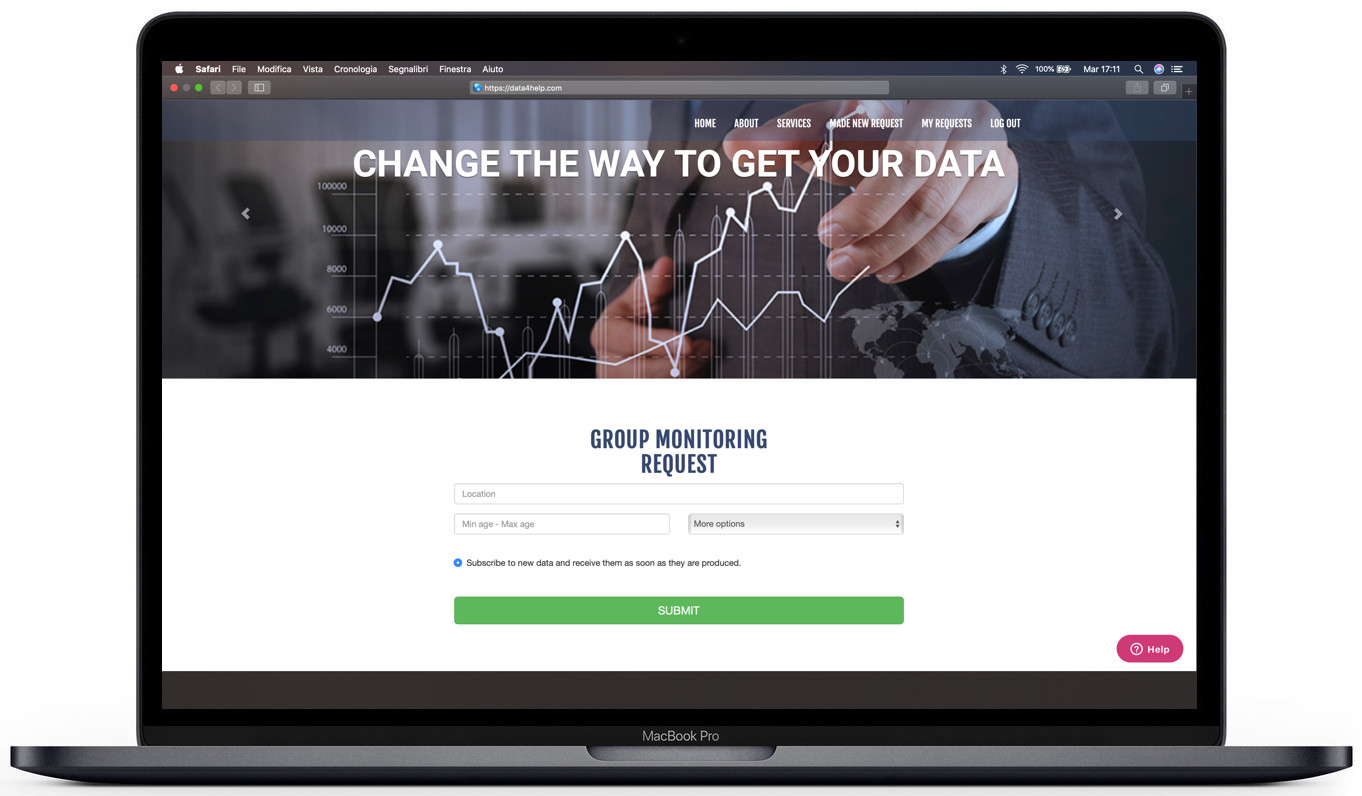
\includegraphics[scale = 0.33]{Images/Mockups/GroupRequest.jpg}
          	\caption{Group Request Form Mockup}
\end{figure}
Otherwise, clicking on {\textcolor{Blue}{\textbf{GROUP MONITORING REQUEST}}} button the system loads a new page containing the form to make a group monitoring request. In the form it is possible to limit the request to a group living in a specific zone, writing the geographical area on the {\textcolor{Blue}{\textbf{Location}}} field. It is then possible to select a minimum and a maximum age. Clicking on the {\textcolor{Blue}{\textbf{More}}} button it is possible to furthermore limit the request adding other filters to the group of individuals. Once the user has filled all the fields, clicking on the {\textcolor{Blue}{\textbf{SUBMIT}}} button the request is forwarded to Data4Help system.
\clearpage

\item[•]{\Large AutomatedSOS}
\bigbreak
\noindent
TrackMe offers to AutomatedSOS users an App for smartwatches, with which the users can see their location and health status information.
\begin{figure}[H]
\begin{center}
        \begin{minipage}[c]{.40\textwidth}
        \centering
          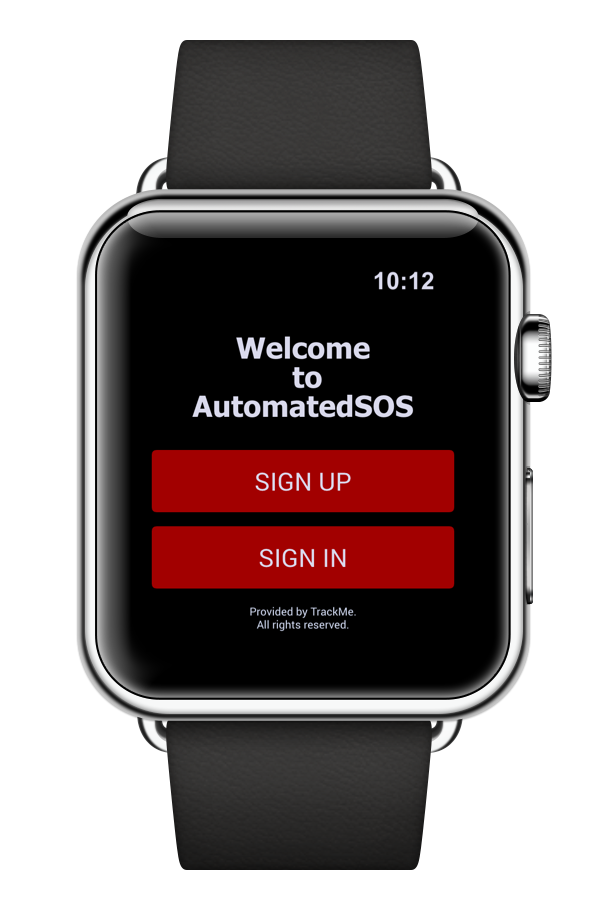
\includegraphics[height=12 cm]{Images/Mockups/AutomatedSOSMockup1.png}
          	\caption{Welcome Page Mockup}
        \end{minipage}%
        \hspace{10mm}%
        \begin{minipage}[c]{.40\textwidth}
        \centering
          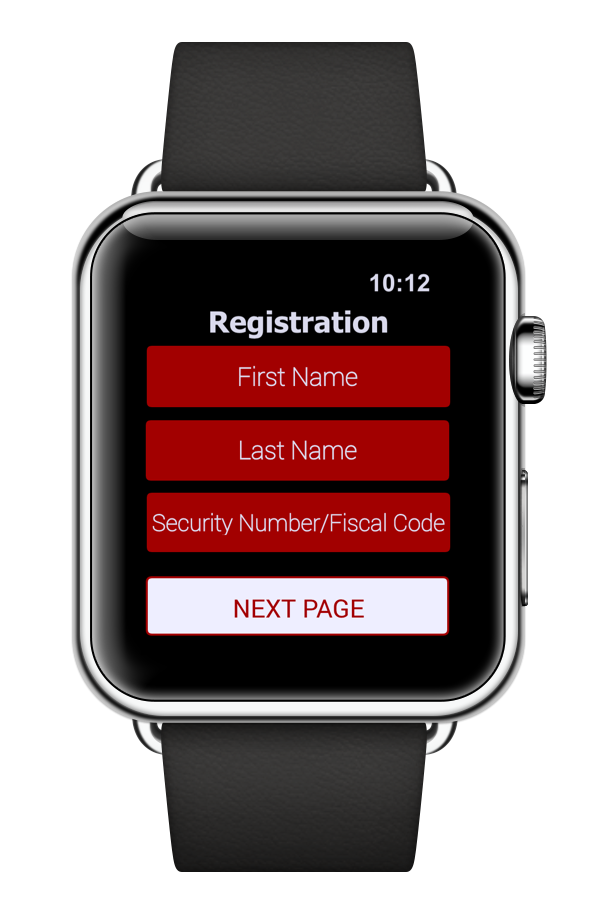
\includegraphics[height=12 cm]{Images/Mockups/AutomatedSOSMockup6.png}
          	\caption{Registration Form Mockup}
        \end{minipage}
      \end{center}
\end{figure}
In the first access to AutomatedSOS App the user is asked to sign up or to sign in 			(Figure 12). Based on the fact that the user could already have a TrackMe account, he/she will choose the right option between the two. In future accesses to the App the user do not need to select each time one of these two possible options because the App automatically remembers the account which is logged in. In case of sign in (Figure 13), the user has to fill all the mandatory fields in order to complete the registration form. Scrolling down the screen other fields will appear. Once every field is correctly filled, it will be possible to select the {\textcolor{Red}{\textbf{NEXT PAGE}}} button. 
\clearpage
\begin{figure}[H]
\begin{center}
        \begin{minipage}[c]{.40\textwidth}
        \centering
          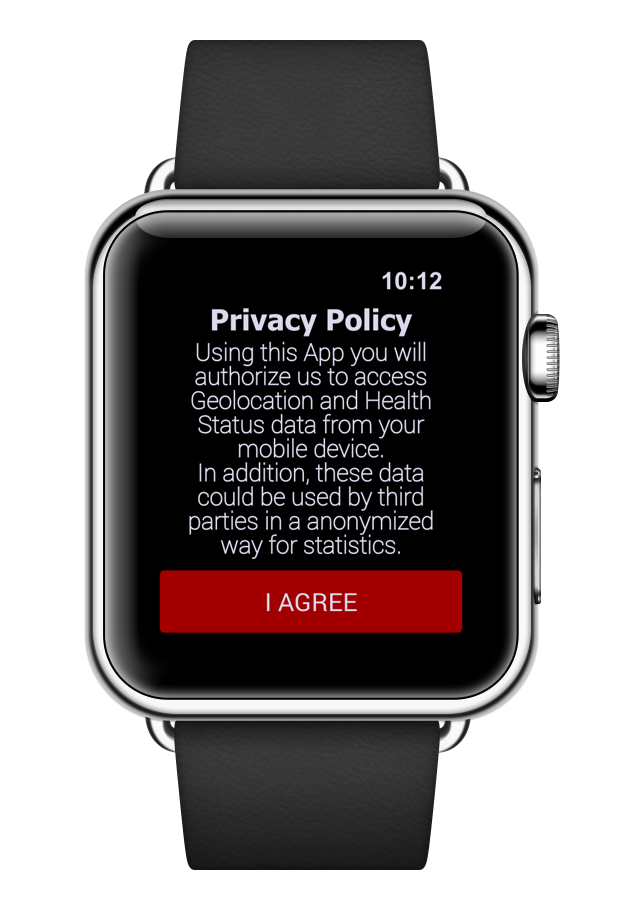
\includegraphics[height=12 cm]{Images/Mockups/AutomatedSOSMockup2.png}
             	\caption{Privacy Policy Conditions Mockup}
        \end{minipage}%
        \hspace{10mm}%
        \begin{minipage}[c]{.40\textwidth}
        \centering
          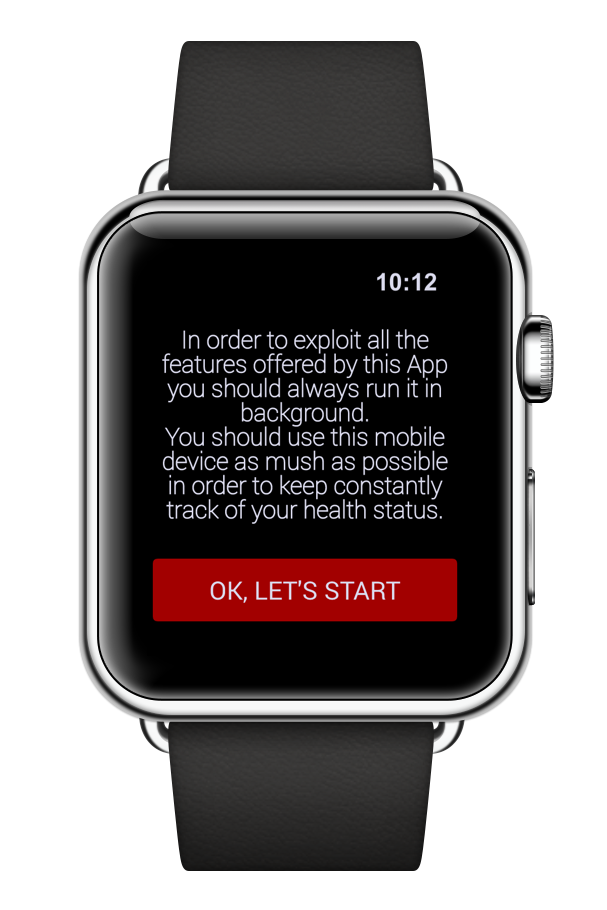
\includegraphics[height=12 cm]{Images/Mockups/AutomatedSOSMockup4.png}
          \vspace{0.1cm}
          	\caption{Usage Conditions Mockup}
        \end{minipage}
      \end{center}
\end{figure}
During the first access to the App, the next step after sign up/sign in is to agree to the Privacy Policy Conditions (Figure 14). In order to use this App the user has to agree to the treatment of Location and Health Status data by Data4Help. In addition, these data could be used by third parties for the group monitoring request. Without agreeing the Privacy Policy Conditions the user cannot go to the next page, therefore he/she will not be able to use this App. Once clicked on {\textcolor{Red}{\textbf{I AGREE}}} the last step before starting using the App is to take note of the importance of wearing the Smartwatch as much as possible and to let the App runs in background (Figure 15).
\clearpage
\begin{figure}
\begin{center}
	\bigbreak
        \begin{minipage}[c]{.40\textwidth}
        \centering
          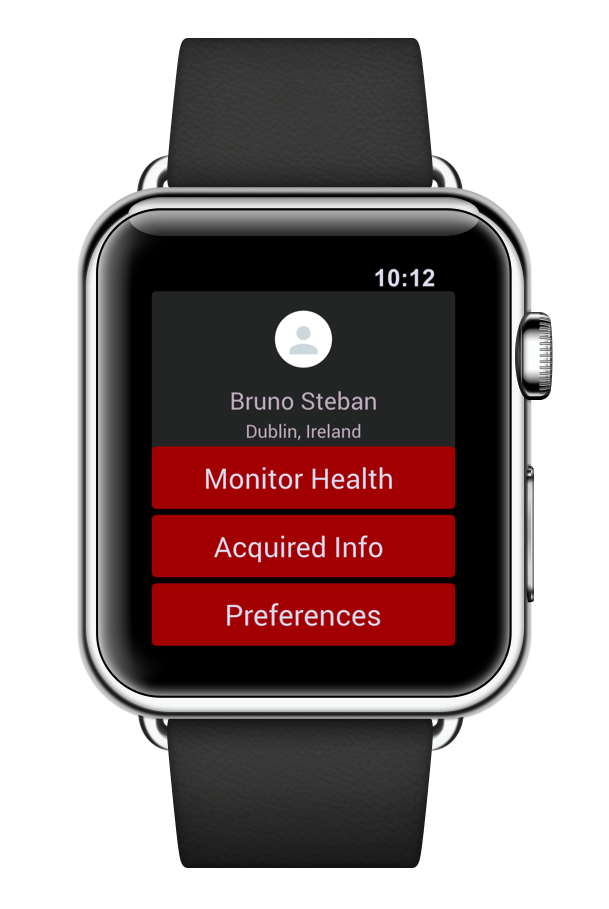
\includegraphics[height=12 cm]{Images/Mockups/AutomatedSOSMockup5.png}
          	\caption{Main Menu Mockup}
        \end{minipage}%
        \hspace{10mm}%
        \begin{minipage}[c]{.40\textwidth}
        \centering
          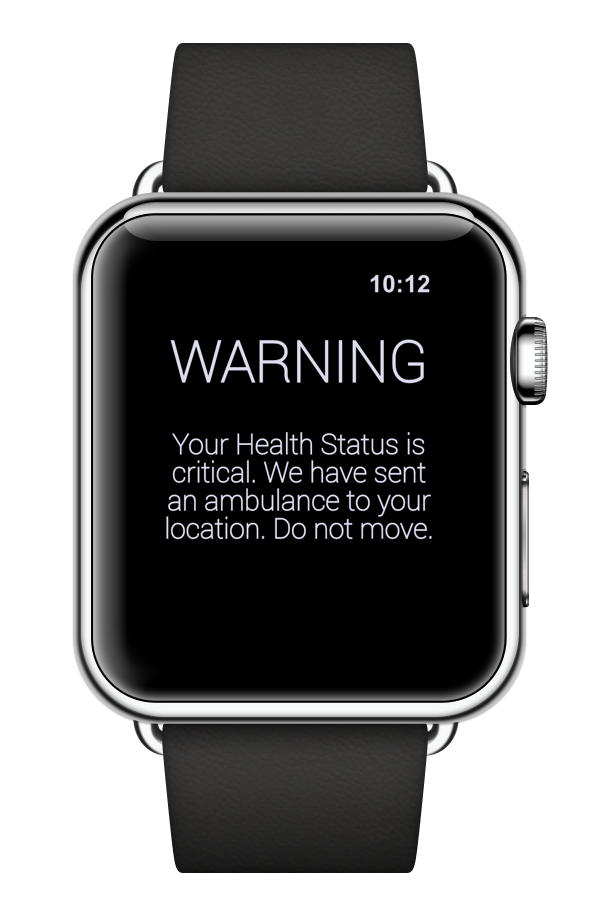
\includegraphics[height=12 cm]{Images/Mockups/AutomatedSOSMockup7.png}
          	\caption{Warning Message Mockup}
        \end{minipage}
      \end{center}
\end{figure}
The main menu of the App, which is immediately accessible by selecting the AutomatedSOS App on the Smartwatch home, is composed by three parts (Figure 16). Selecting {\textcolor{Red}{\textbf{Monitor Health}}} the user can see live health information, like the current Heart Rate, Blood Pressure and so on. Choosing the {\textcolor{Red}{\textbf{Acquired Info}}} button the user can see all the historical data stored since the first access to the App. Finally, {\textcolor{Red}{\textbf{Preferences}}} option allows the user to set his/her own threshold parameters according to the particular illnesses he/she is affected, own age and so on. As soon as an ambulance request is sent and acknowledged due to the user's critical health status a warning message (Figure 17) appears on the screen of the smartwatch notified by an alert sound.
\clearpage

\item[•]{\Large Track4Run}
\bigbreak
\noindent
Track4Run users can use an App for smartphone and another one for smartwatches. The first one could be used by everyone, while the second one is made only for the athletes.
\\[0.5 cm]
\begin{figure}[H]
\begin{center}
        \begin{minipage}[c]{.40\textwidth}
        \centering
          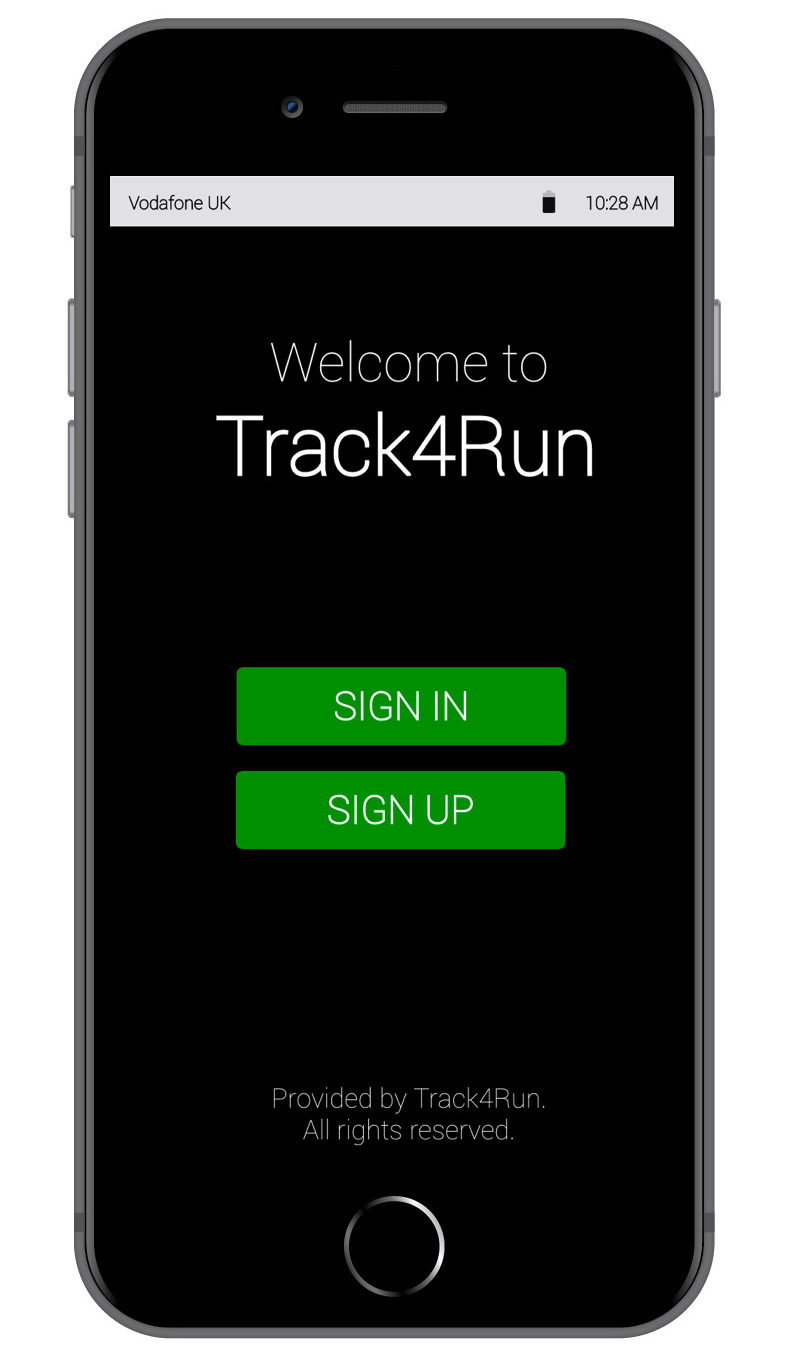
\includegraphics[height=14 cm]{Images/Mockups/Track4RunMockup1.jpg}
	\caption{Welcome Page Mockup}
        \end{minipage}%
        \hspace{10mm}%
        \begin{minipage}[c]{.40\textwidth}
        \centering
          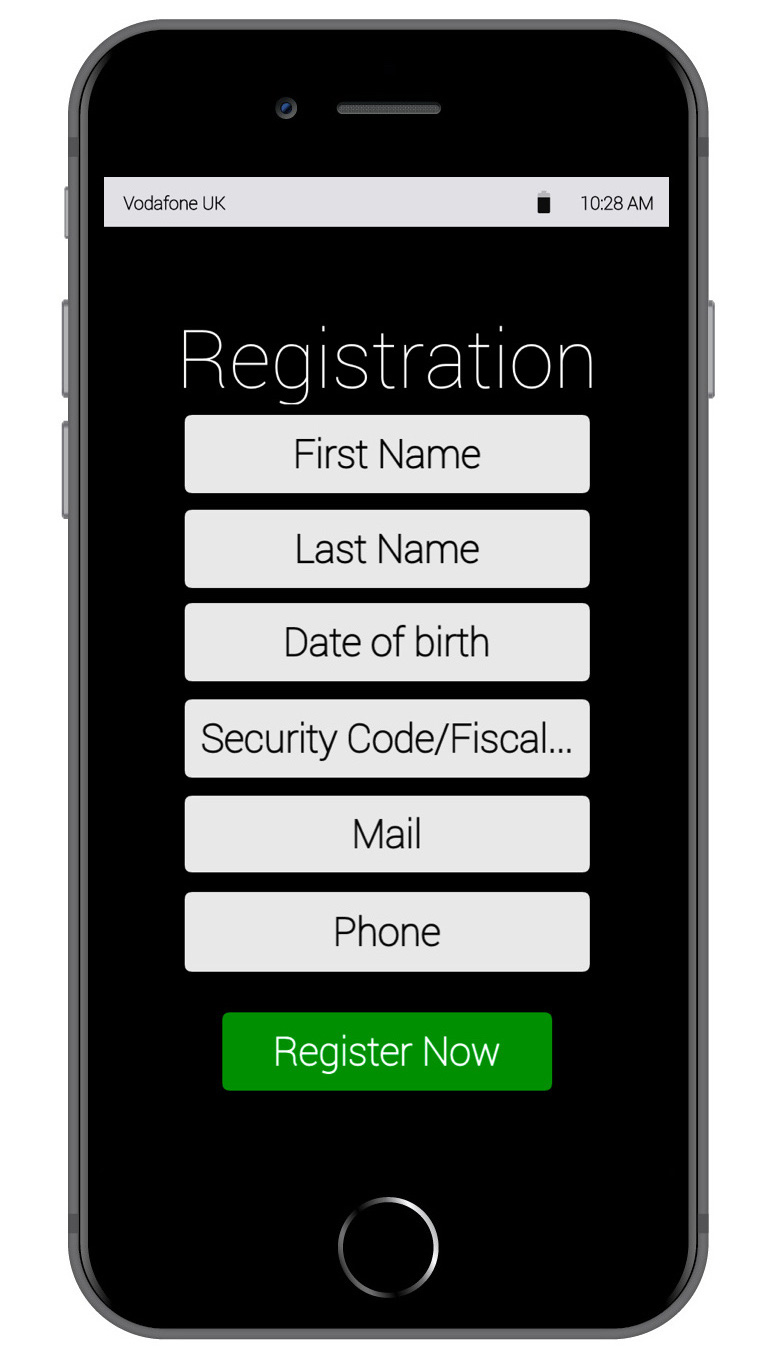
\includegraphics[height=14 cm]{Images/Mockups/Track4RunMockup4.jpg}
	\caption{Registration Form Mockup}
        \end{minipage}
      \end{center}
\end{figure}
In the first access to Track4Run App the user is asked to sign up or to sign in 			(Figure 18). Based on the fact that the user could already have a TrackMe account he/she will choose the right option between the two. In future accesses to the App the user do not need to select each time one of these two possible options because the App automatically remembers the account which is logged in. In case of sign in (Figure 19), the user has to fill all the mandatory fields in order to complete the registration form. Once every field is correctly filled, it will be possible to complete the registration selecting the {\textcolor{Green}{\textbf{Register Now}}} button. 
\clearpage
\begin{figure}[H]
\begin{center}
        \begin{minipage}[c]{.40\textwidth}
        \centering
          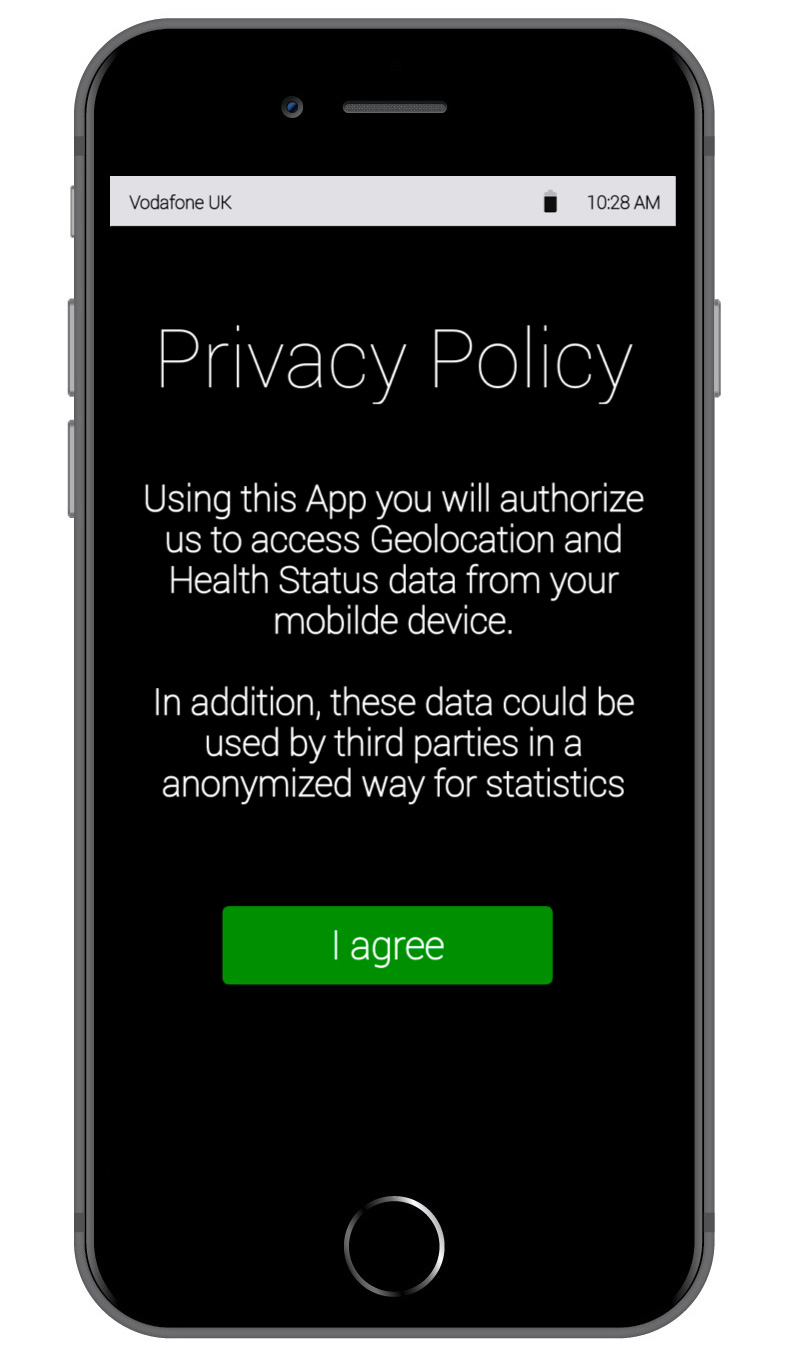
\includegraphics[height=14 cm]{Images/Mockups/Track4RunMockup2.jpg}
	\caption{Privacy Policy Conditions pt.1 Mockup}
        \end{minipage}%
        \hspace{10mm}%
        \begin{minipage}[c]{.40\textwidth}
        \centering
          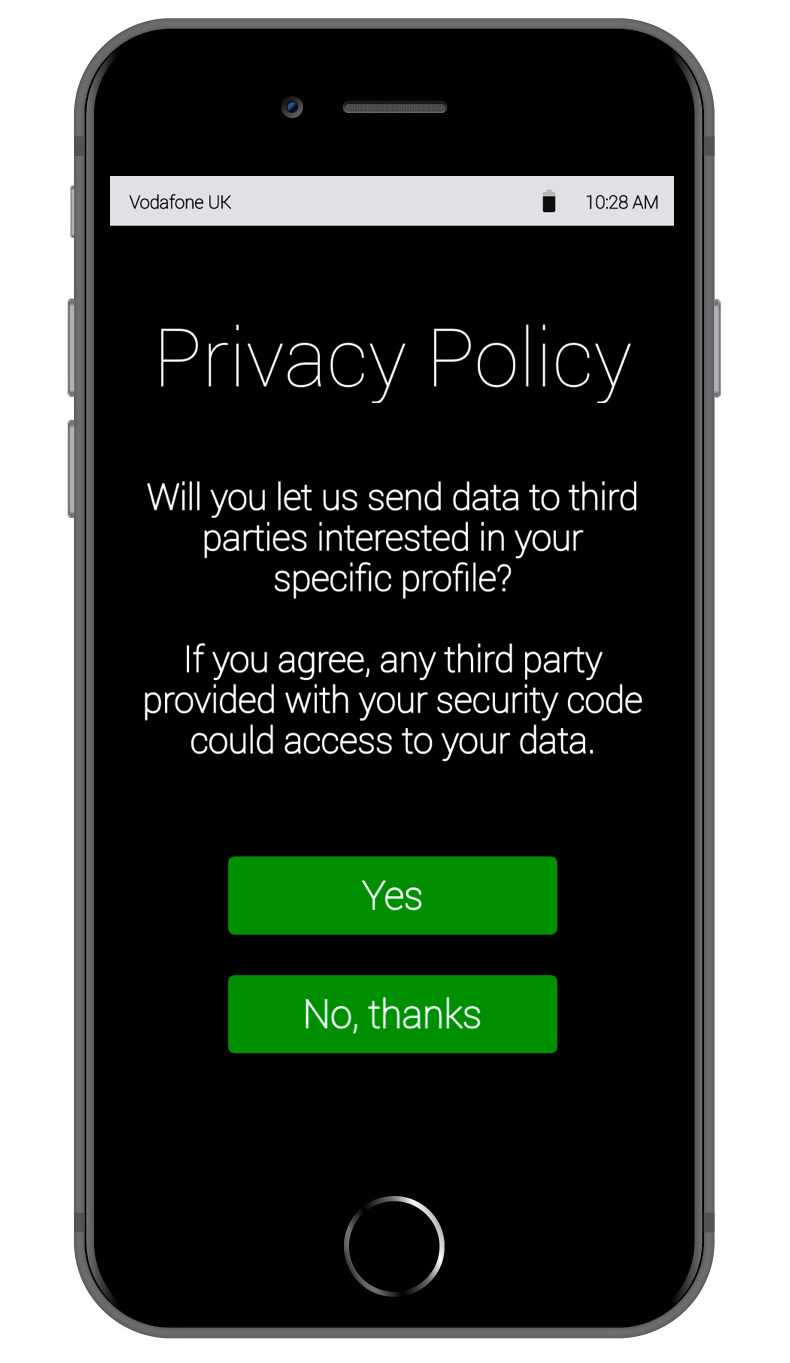
\includegraphics[height=14 cm]{Images/Mockups/Track4RunMockup3.jpg}
	\caption{Privacy Policy Conditions pt.2 Mockup}
        \end{minipage}
      \end{center}
\end{figure}
During the first access to the App, the next step after sign up/sign in is to agree the Privacy Policy Conditions (Figure 20). In order to use this App the user has to agree the treatment of Location and Health Status data by Data4Help. In addition, these data could be used by third parties for the group monitoring request. Without agreeing the Privacy Policy Conditions the user can not go to the next page, therefore he/she will not be able to use this App. All the three first steps presented so far are substantially the same of AutomatedSOS. The next step regards the second part of the Privacy Policy Conditions (which was not presented for the previous system) about individual monitoring request (Figure 21).  In this case it is not strictly necessary to accept it, the user simply can select the {\textcolor{Green}{\textbf{No, thanks}}} option.
\clearpage
\begin{figure}[H]
\begin{center}
        \begin{minipage}[c]{.40\textwidth}
        \centering
          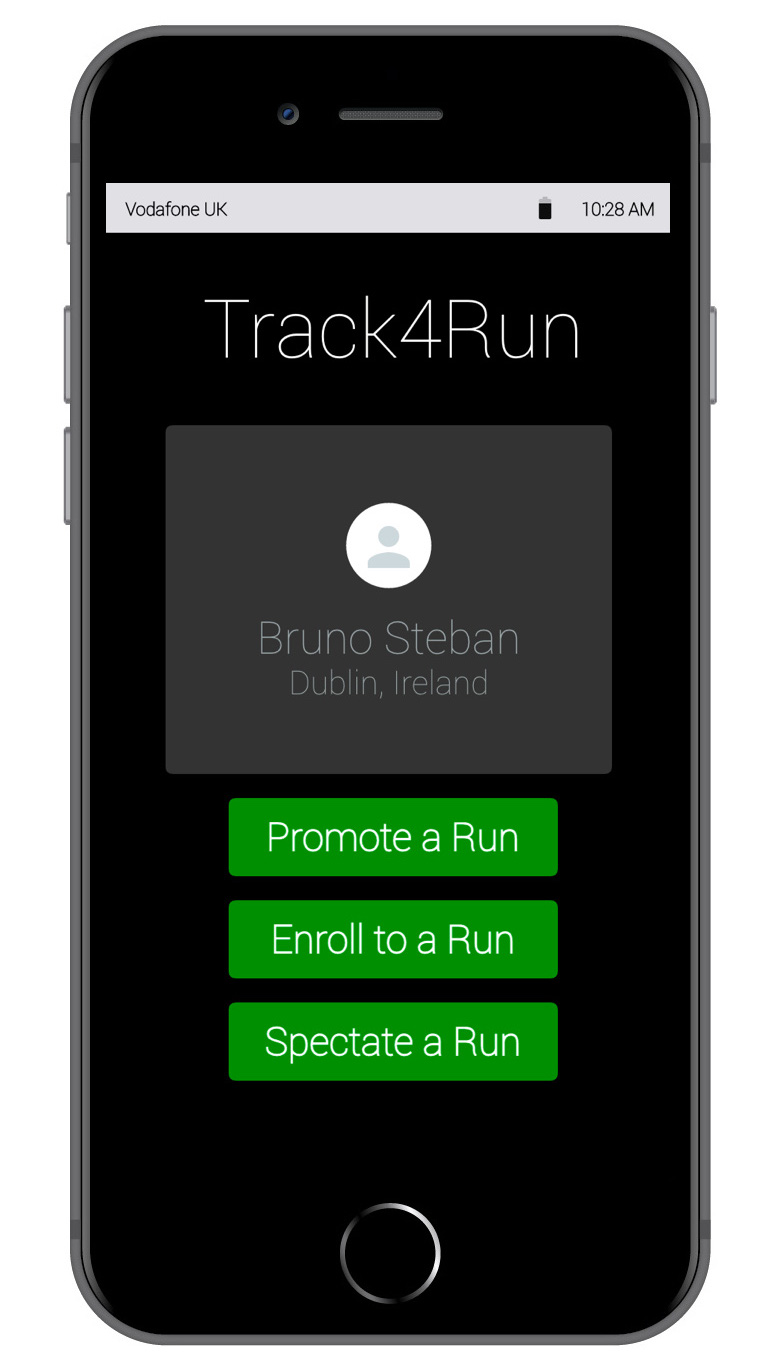
\includegraphics[height=14 cm]{Images/Mockups/Track4RunMockup5.jpg}
	\caption{Main Menu Mockup}
        \end{minipage}%
        \hspace{10mm}%
        \begin{minipage}[c]{.40\textwidth}
        \centering
          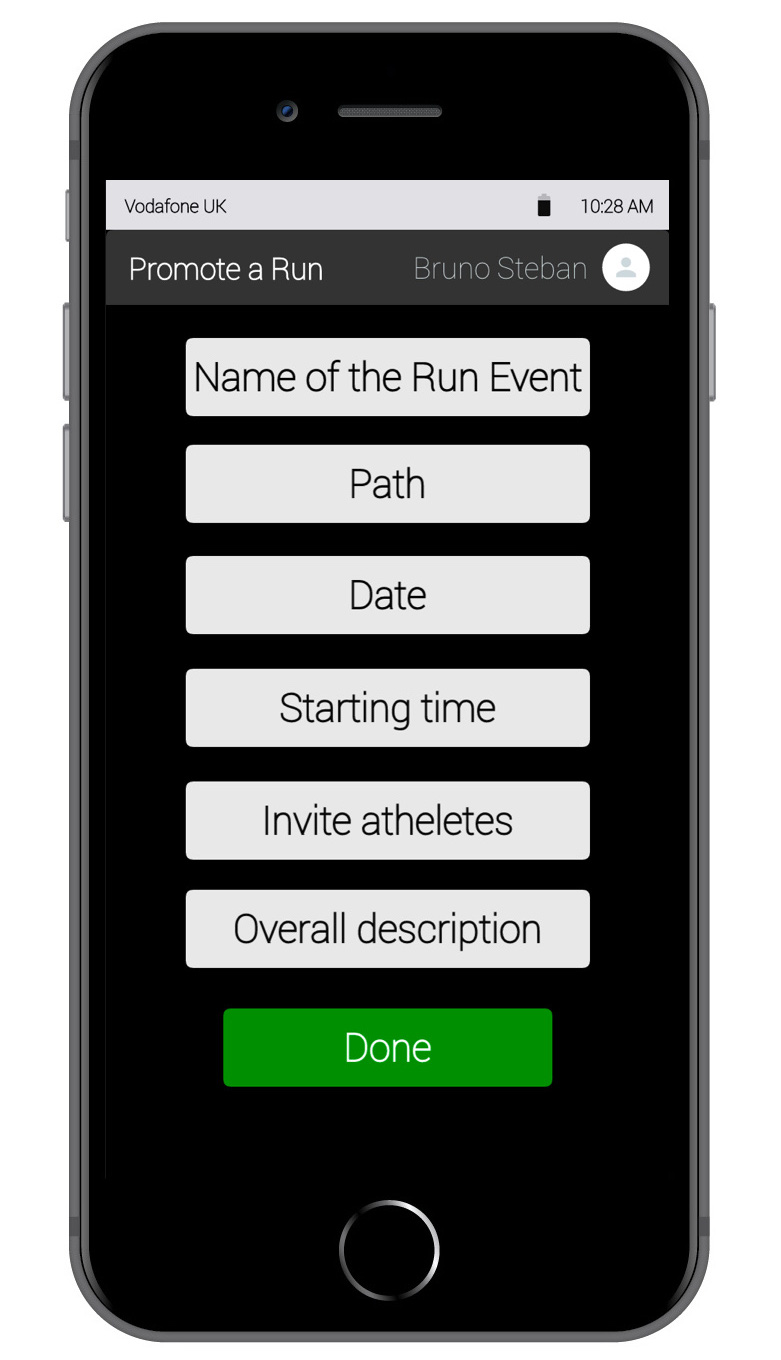
\includegraphics[height=14 cm]{Images/Mockups/Track4RunMockup6.jpg}
	\caption{Promote a Run View Mockup}
        \end{minipage}
      \end{center}
\end{figure}
In Track4Run Home three options are possible (Figure 22). Selecting the first one, {\textcolor{Green}{\textbf{Promote a Run}}}, a user can create a run event and promote it inviting athletes. The second option, which is {\textcolor{Green}{\textbf{Enroll to a Run}}} allows the user to enroll to a run. Finally, choosing {\textcolor{Green}{\textbf{Spectate a Run}}} the user can see on a map the position of all athletes during the run. Now, we analyze these three possibilities in detail. Choosing the first one the App leads the user to a new page in order to manage the event (Figure 23). Here, it is possible to set all the necessary features of the run, like defining the path on a map, setting the date, the starting time and so on. It is also possible to invite athletes to the run in order to promote the event.
\clearpage
\begin{figure}[H]
\begin{center}
        \begin{minipage}[c]{.40\textwidth}
        \centering
          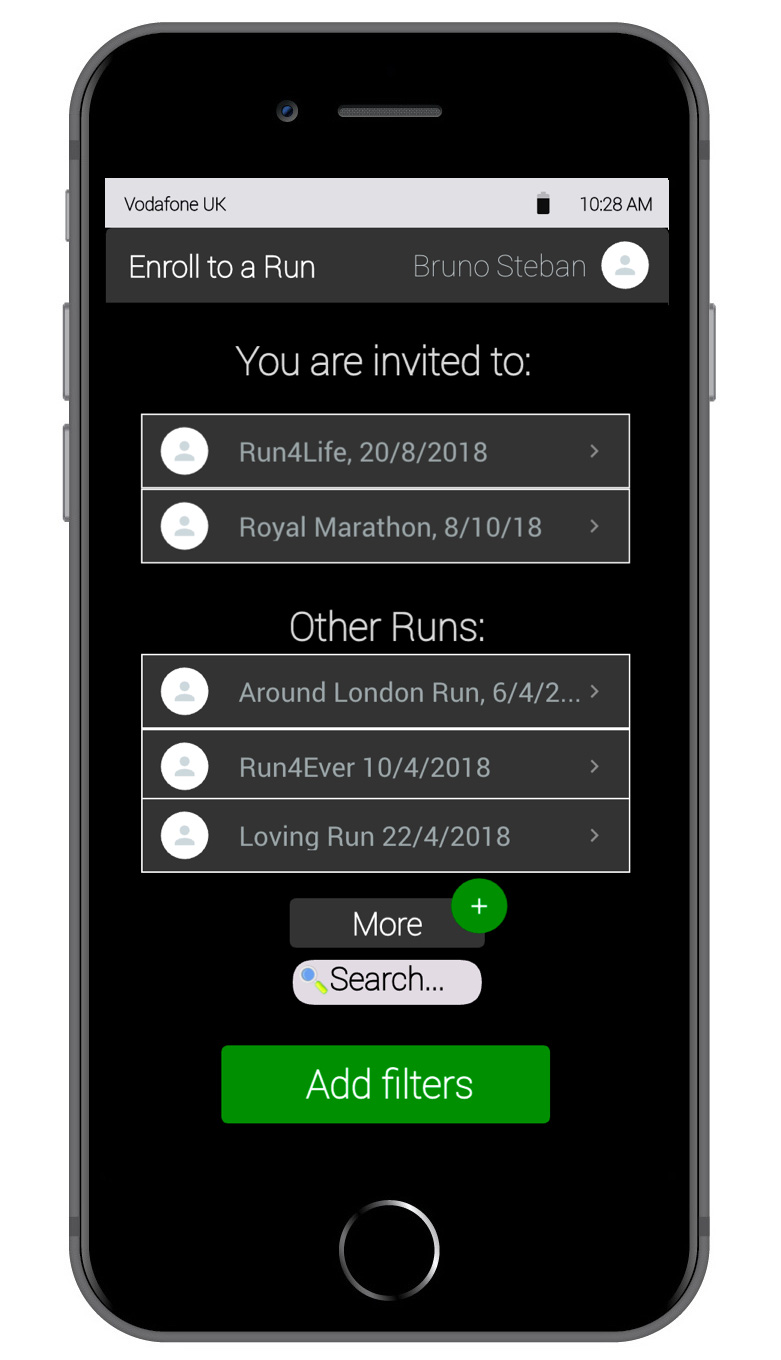
\includegraphics[height=14 cm]{Images/Mockups/Track4RunMockup7.jpg}
	\caption{Enroll to a Run View Mockup}
        \end{minipage}%
        \hspace{10mm}%
        \begin{minipage}[c]{.40\textwidth}
        \centering
          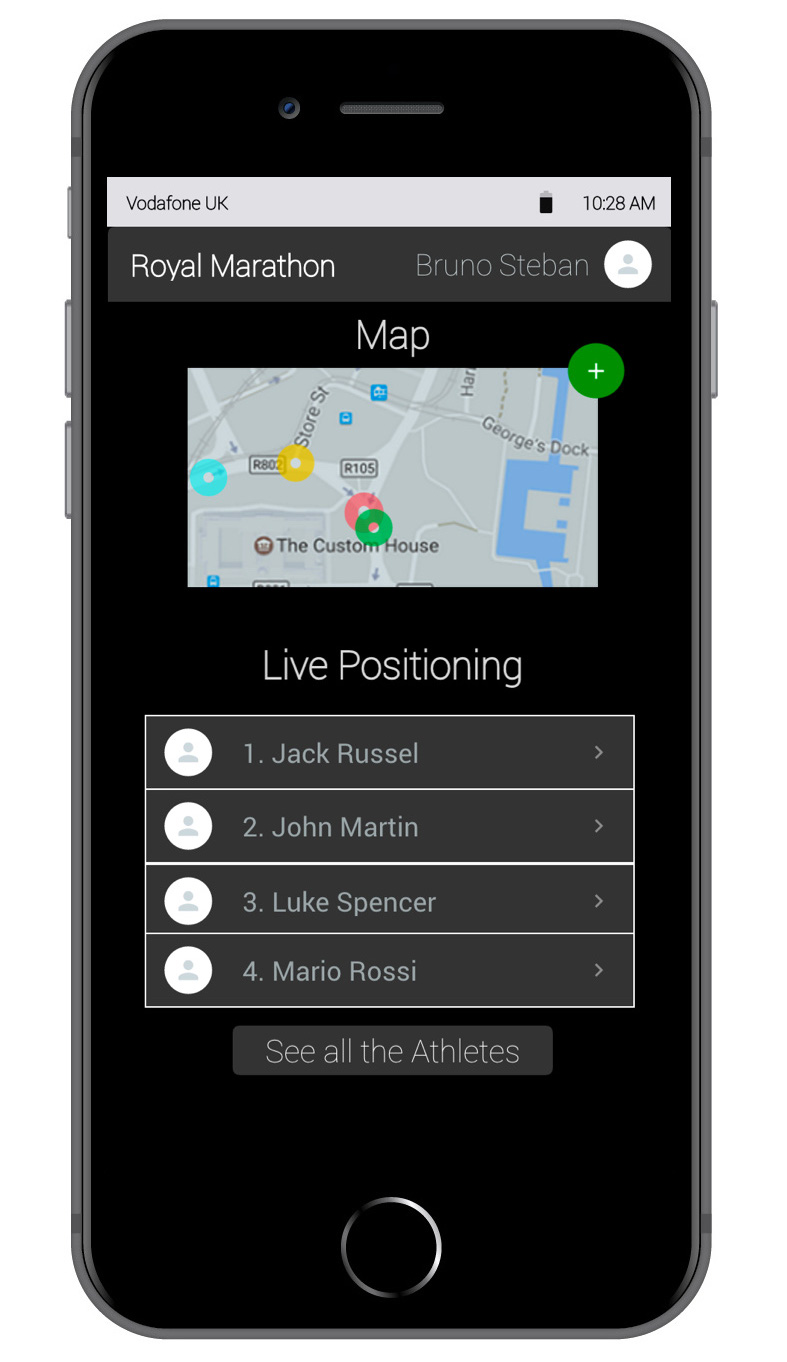
\includegraphics[height=14 cm]{Images/Mockups/Track4RunMockup8.jpg}
	\caption{Spectate a Run View Mockup}
        \end{minipage}
      \end{center}
\end{figure}
In the section Enroll to a Run (Figure 24) a user can see a list of all the runs in which he/she has been invited to. The user can select one of these runs to see furthermore details about it and at the end to enroll to it. A list of all the runs that will be soon held is showed immediately below. Since the large number of all the future runs, only a little portion of them is showed, selecting the {\textcolor{Green}{\textbf{More +}}} button the user can see another set of run events. In addition, through {\textcolor{Green}{\textbf{Add filters}}} it is possible to limit the list of the all runs to a specific date, location and similar options. To easily access to a specific run, the {\textcolor{Green}{\textbf{Search}}} button allows the user to immediately find the run he/she was looking for. In the last section, Spectate a Run (Figure 25), it is possible to spectate a specific run in an interactive way. A map shows all the runners enrolled in it, each one represented by a different colored circle. Selecting the {\textcolor{Green}{\textbf{+}}} button is possible to zoom in the map that will appear on full-screen mode. Below the map the live positioning shows the first four athletes, anyway selecting {\textcolor{Green}{\textbf{See all the Athletes}}} option it is possible to see the live positions of all the participants.
\clearpage
\end{enumerate}